\chapter{Ordering in Inherent Structures}

In the previous chapter we investigated the dynamics of three molecular systems. The dynamics properties of these systems remained smooth throughout the range we simulated them, indicating that there was no phase transition taking place. While there is no obvious phase transition, one possible cause of the increasing time scales for the dynamics properties is the growth of crystal regions within the simulations.

The goal of this chapter is to investigate the structural properties of the three systems studied in the previous chapter to determine whether the dynamic properties observed are purely dynamic properties or can be attributed to structural properties of the system.

\section{Is there Crystal Formation}

Over the course of the simulations to determine the dynamic properties of the system it is possible that the system transitioned from the purely amorphous phase to a structure that was a mixture of crystalline and amorphous regions. If these regions are long lived, rather than just fluctuations, as the temperature is dropped these regions are only more likely to grow; the lower entropy crystal phase is more favourable at low temperatures. Using this reasoning we can use the final configuration as an indication of the formation of crystalline regions over the entire temperature range of the simulation. From this final configuration we can take an inherent structure, removing any of the vibrational noise giving a configuration that is representative of the mean arrangement of the molecules. These arrangements are shown in \textfigref{inherent structures frame} where the colour of each molecule is given by its orientation.
\towrite{discuss inherent structures}

\begin{figure}
    \todofigure{Inherent structures}
    \caption{Inherent structures}
    \label{fig:inherent structures frame}
\end{figure}

While there appears to be no long range ordering in these configurations, to make a definitive statement we need more specialised tools. Consider the compact binary packing with a size ration of 0.637556:1; this is equivalent to packing the \scon molecule without the allocation of bonds. The allocation of bonds can be performed randomly with no adjustment to the structure of the underlying particles~\secref{compact degeneracy}. Two examples of assigning bonds; an ordered p2 structure~\figref{ordered frame}, and a randomly oriented structure~\figref{random frame}. The orientational order of the p2 structure can easily be seen with diagonal banding of colours, corresponding to the two orientations present in the structure. The randomly assigned structure has molecules arranged with no orientational order, distributed between the eight possible molecular orientations. We can attempt to remove the noise of this orientational disorder by only plotting the centers of mass~\figref{ordered com, random com}, however this gives a very similar result, the ordered structure exhibits distinctly crystalline behaviour with centers of mass aligning in rows while the random structure that needs further analysis to be considered ordered.

Both of the previous attempts at describing order in the compact packing were using the properties of a molecule, its orientation and center of mass. While molecular properties are useful for dynamics, in both the ordered and random allocation of bonds the molecule is just a construct sitting atop a lattice of ordered particles. The particles define the arrangement and so using the particles to detect order within a configuration is a far more appropriate approach. Using the particles to define a 2D radial distribution function gives \textfigref{ordered radial2d, random radial2d} which are almost identical to each other. The energy and ordering of the structures is determined by the arrangement of the individual particles, not the arrangement of bonds.

\begin{figure}
    \begin{subfigure}{0.5\textwidth}
        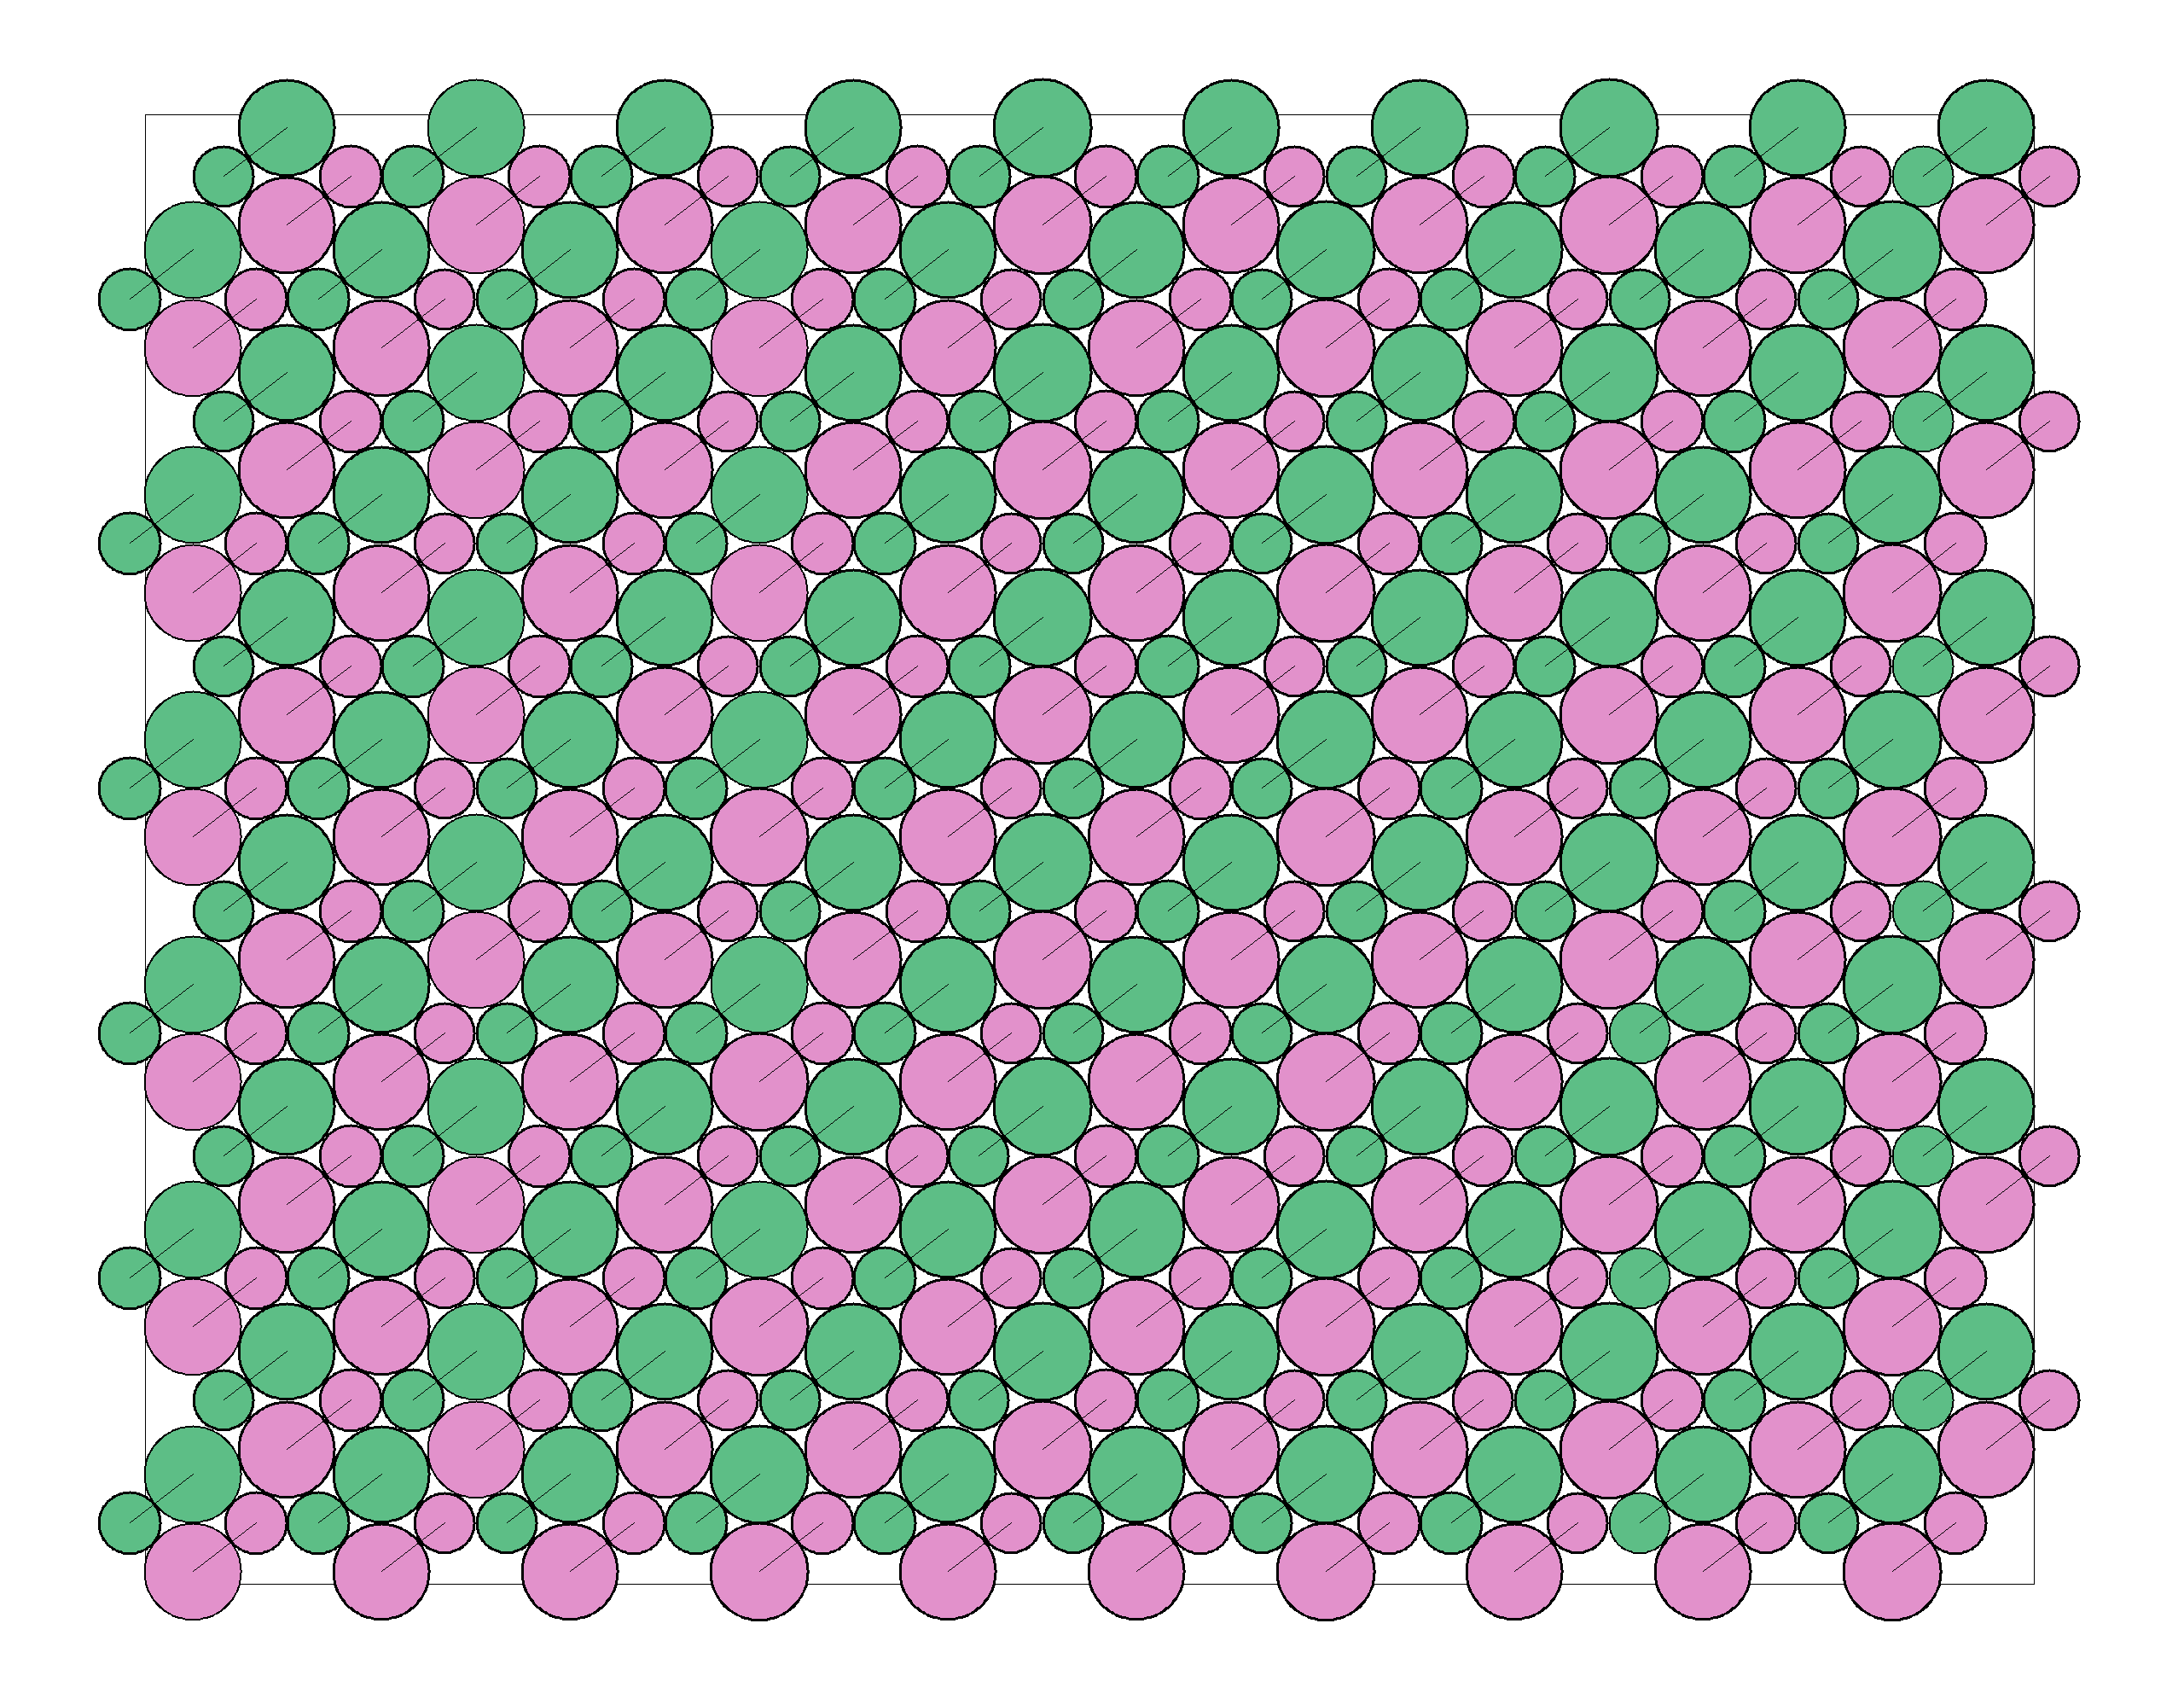
\includegraphics[width=\textwidth]{ordered-frame}
        \caption{Ordered frame}
        \label{fig:ordered frame}
    \end{subfigure}
    \begin{subfigure}{0.5\textwidth}
        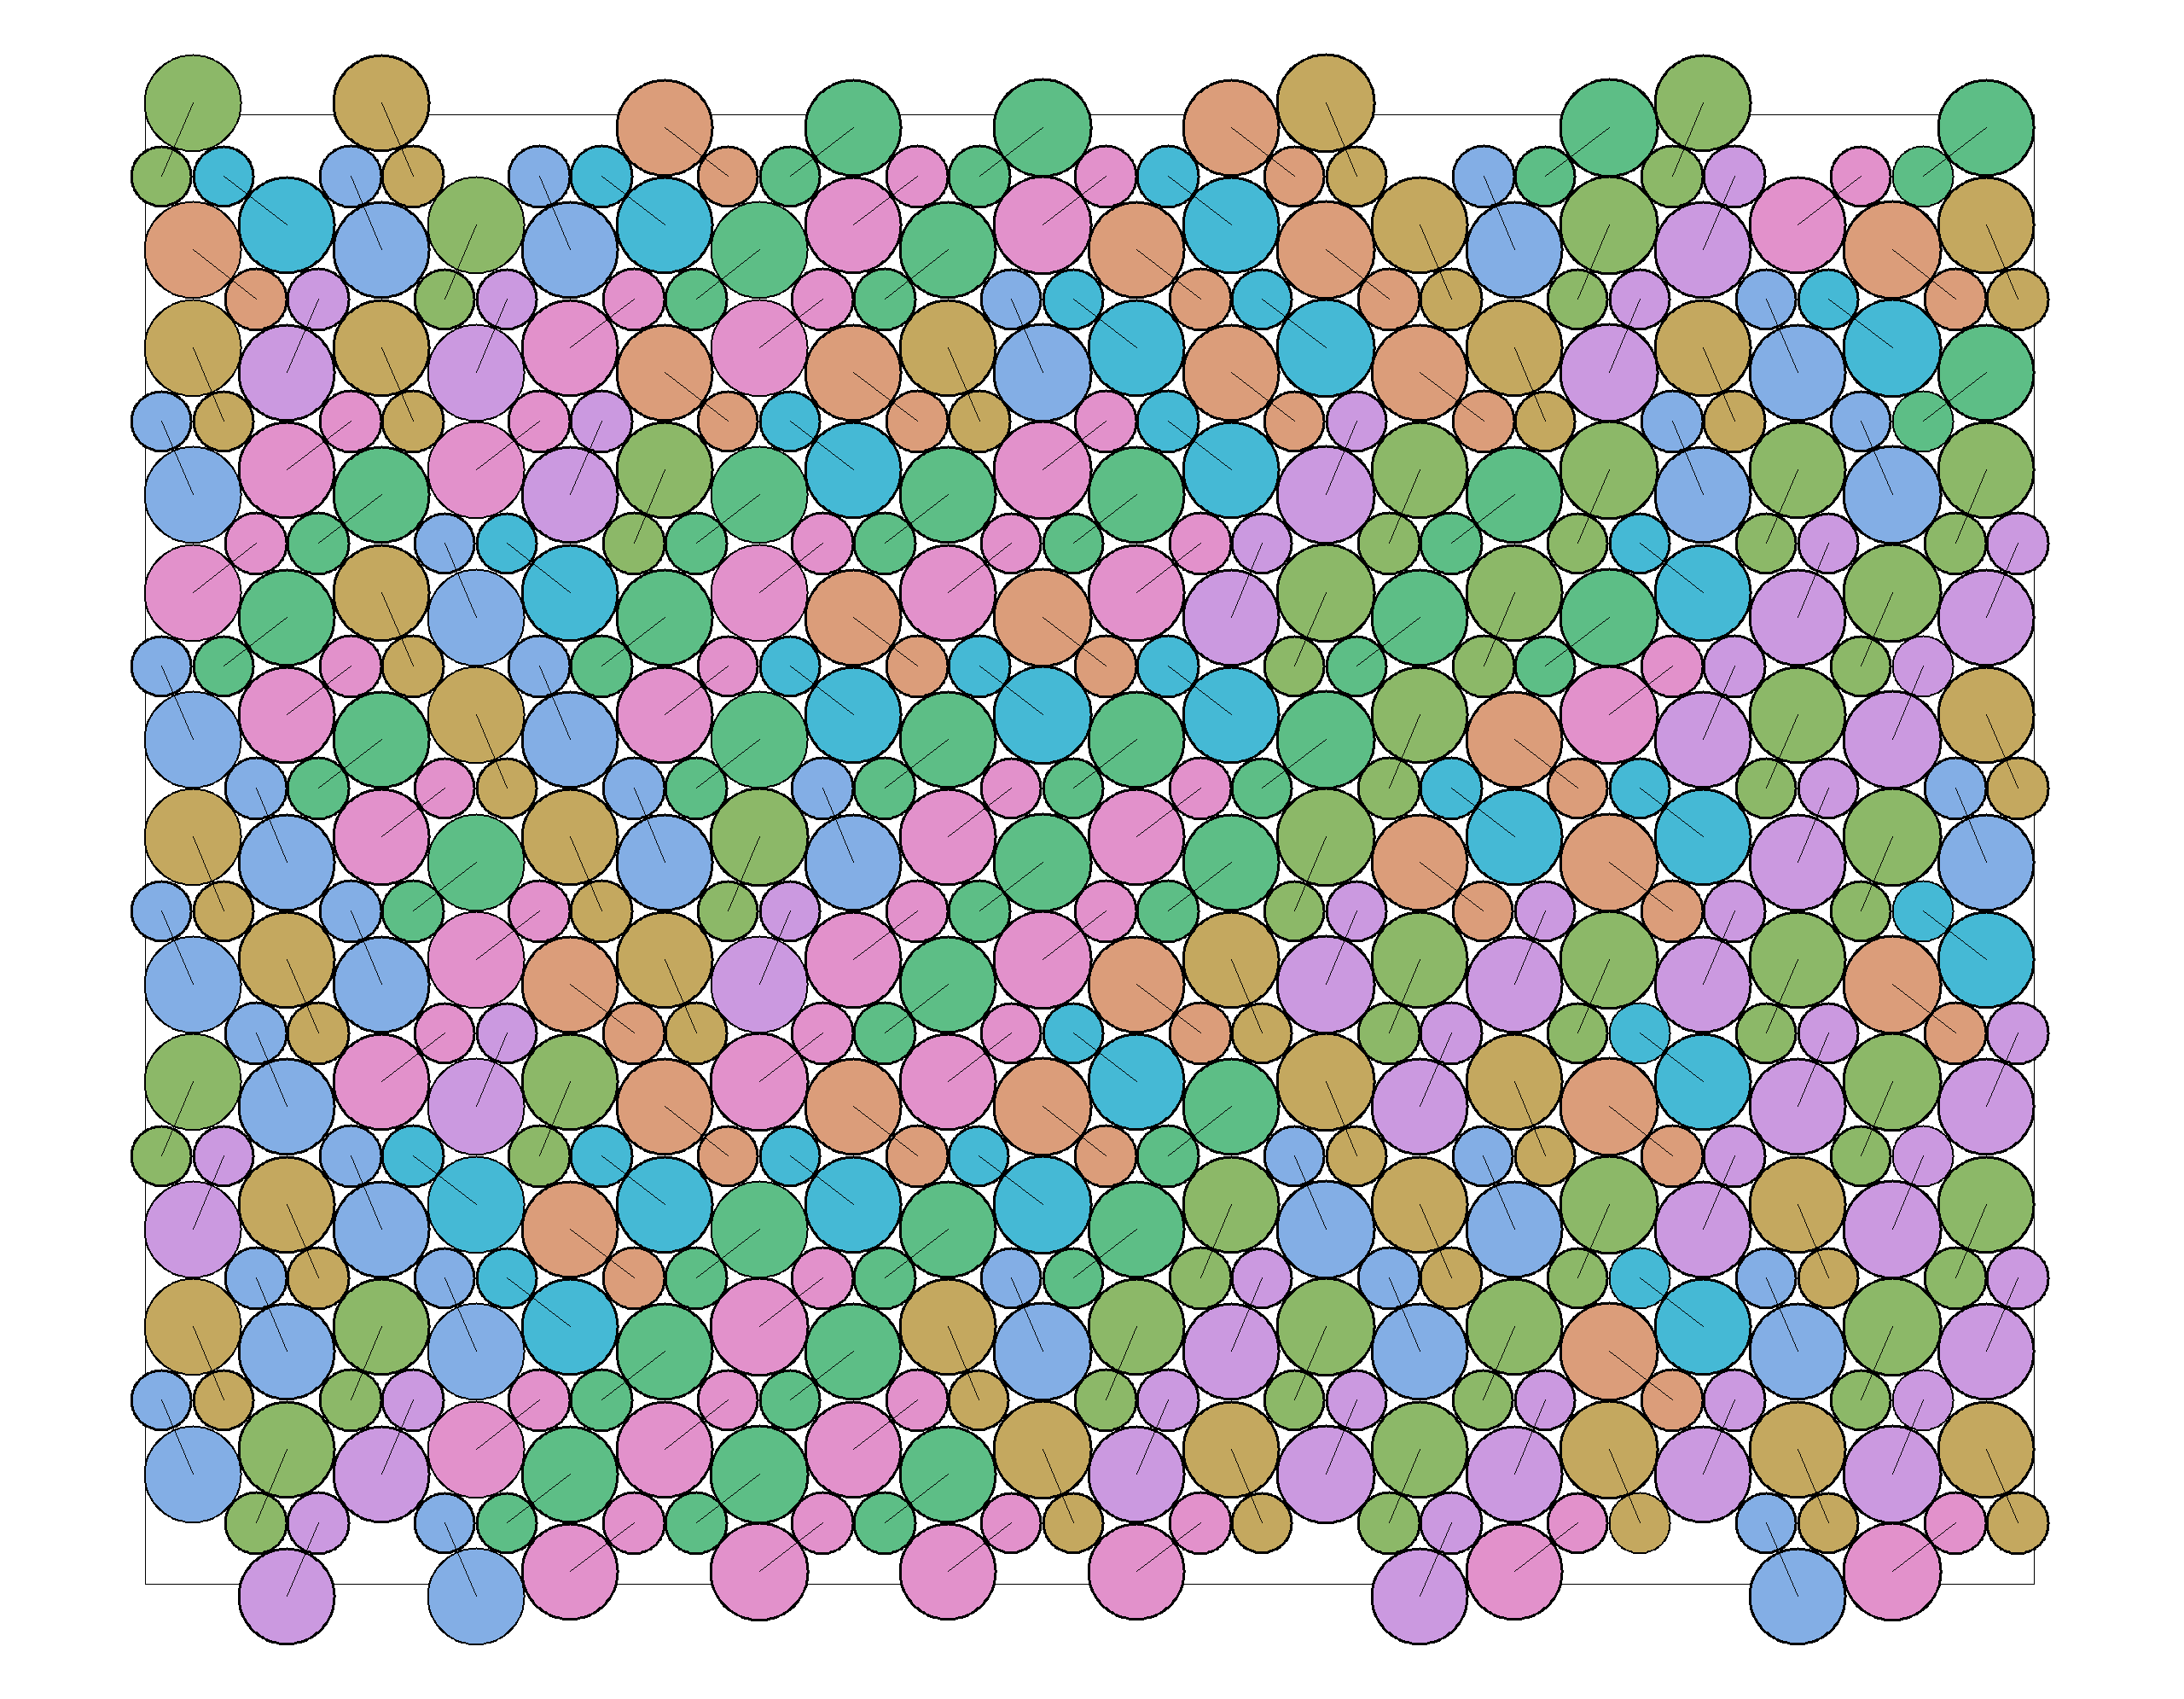
\includegraphics[width=\textwidth]{random-frame}
        \caption{Random frame}
        \label{fig:random frame}
    \end{subfigure}
    \begin{subfigure}{0.5\textwidth}
        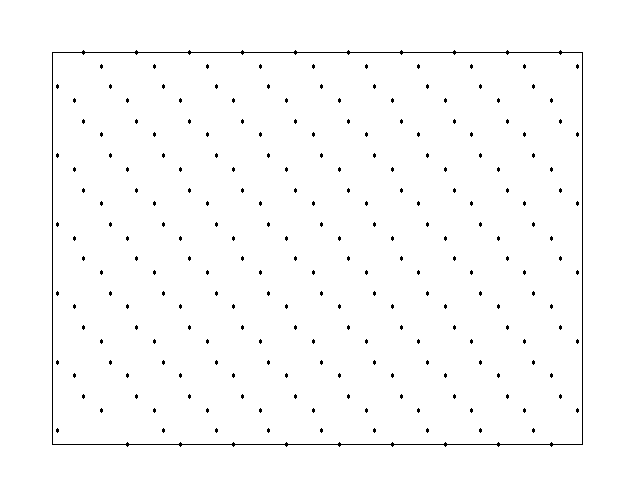
\includegraphics[width=\textwidth]{ordered-com}
        \caption{Ordered com}
        \label{fig:ordered com}
    \end{subfigure}
    \begin{subfigure}{0.5\textwidth}
        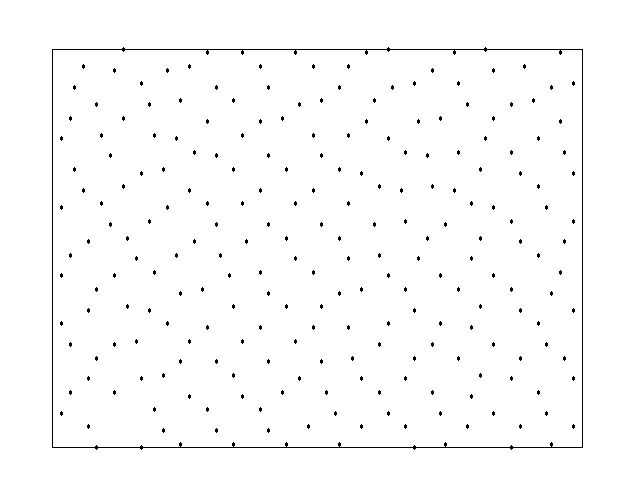
\includegraphics[width=\textwidth]{random-com}
        \caption{Random com}
        \label{fig:random com}
    \end{subfigure}
    \begin{subfigure}{0.5\textwidth}
        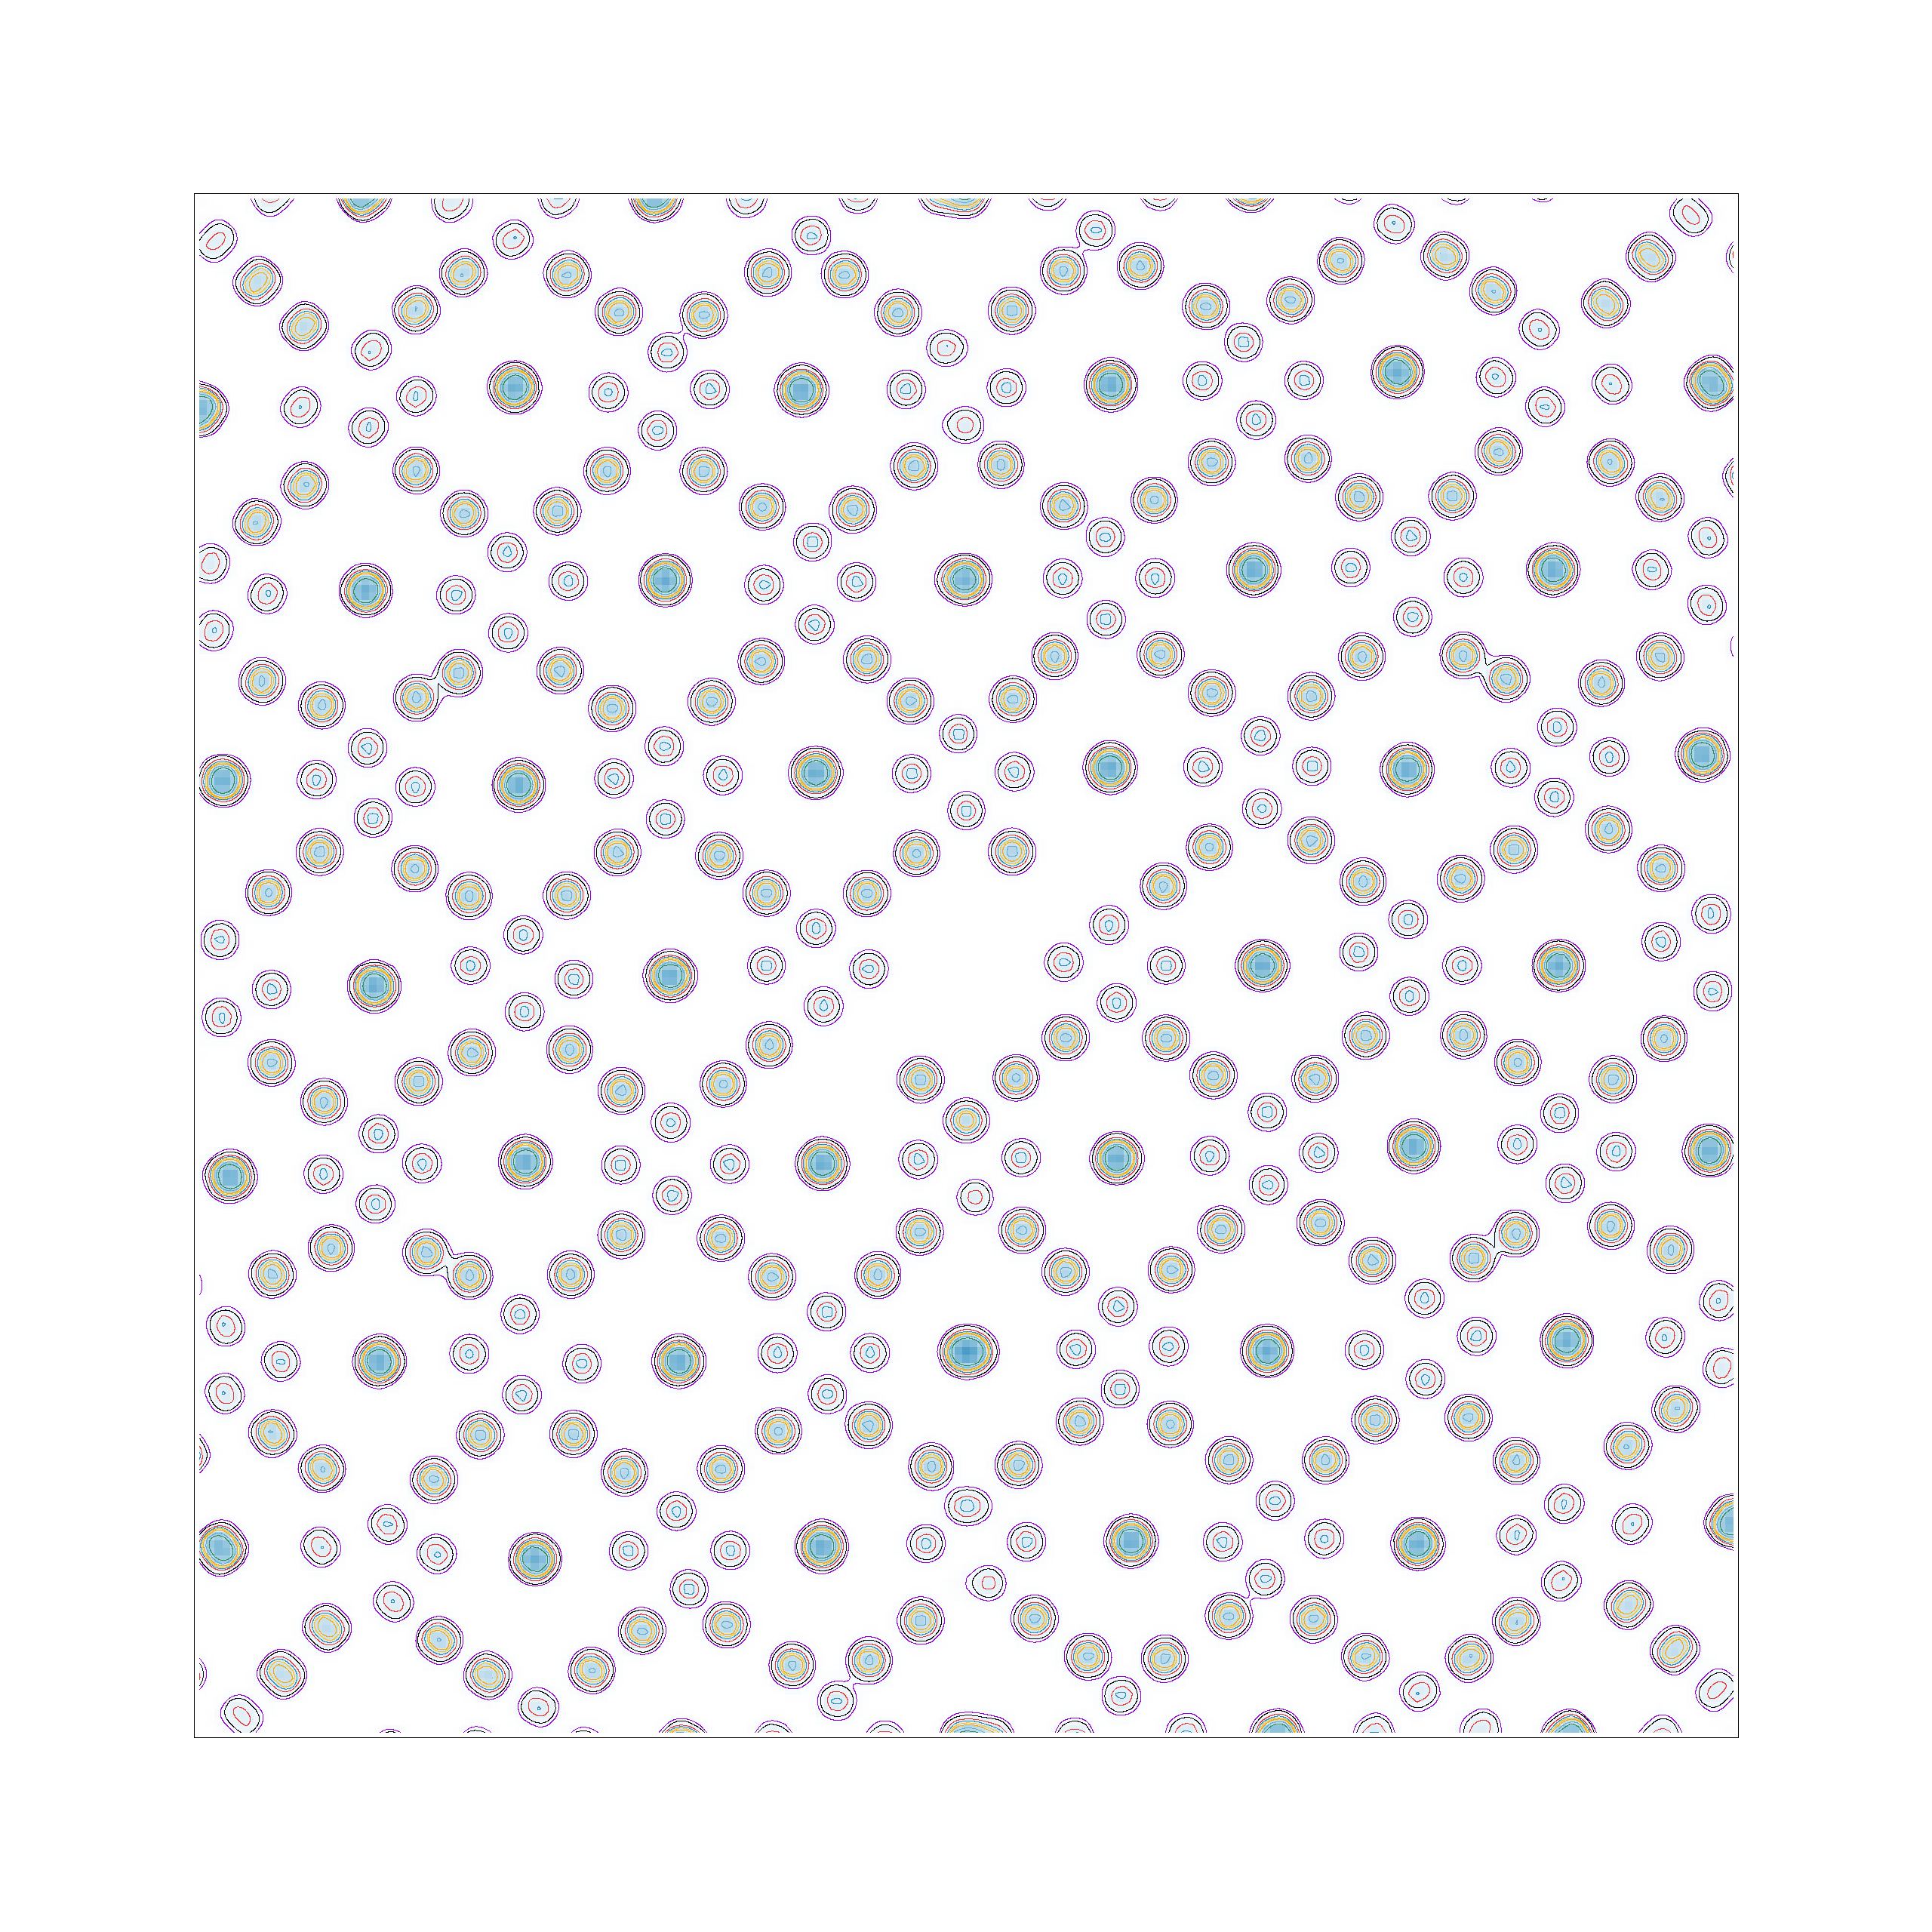
\includegraphics[width=\textwidth]{ordered-radial2d-part}
        \caption{Ordered radial2d}
        \label{fig:ordered radial2d}
    \end{subfigure}
    \begin{subfigure}{0.5\textwidth}
        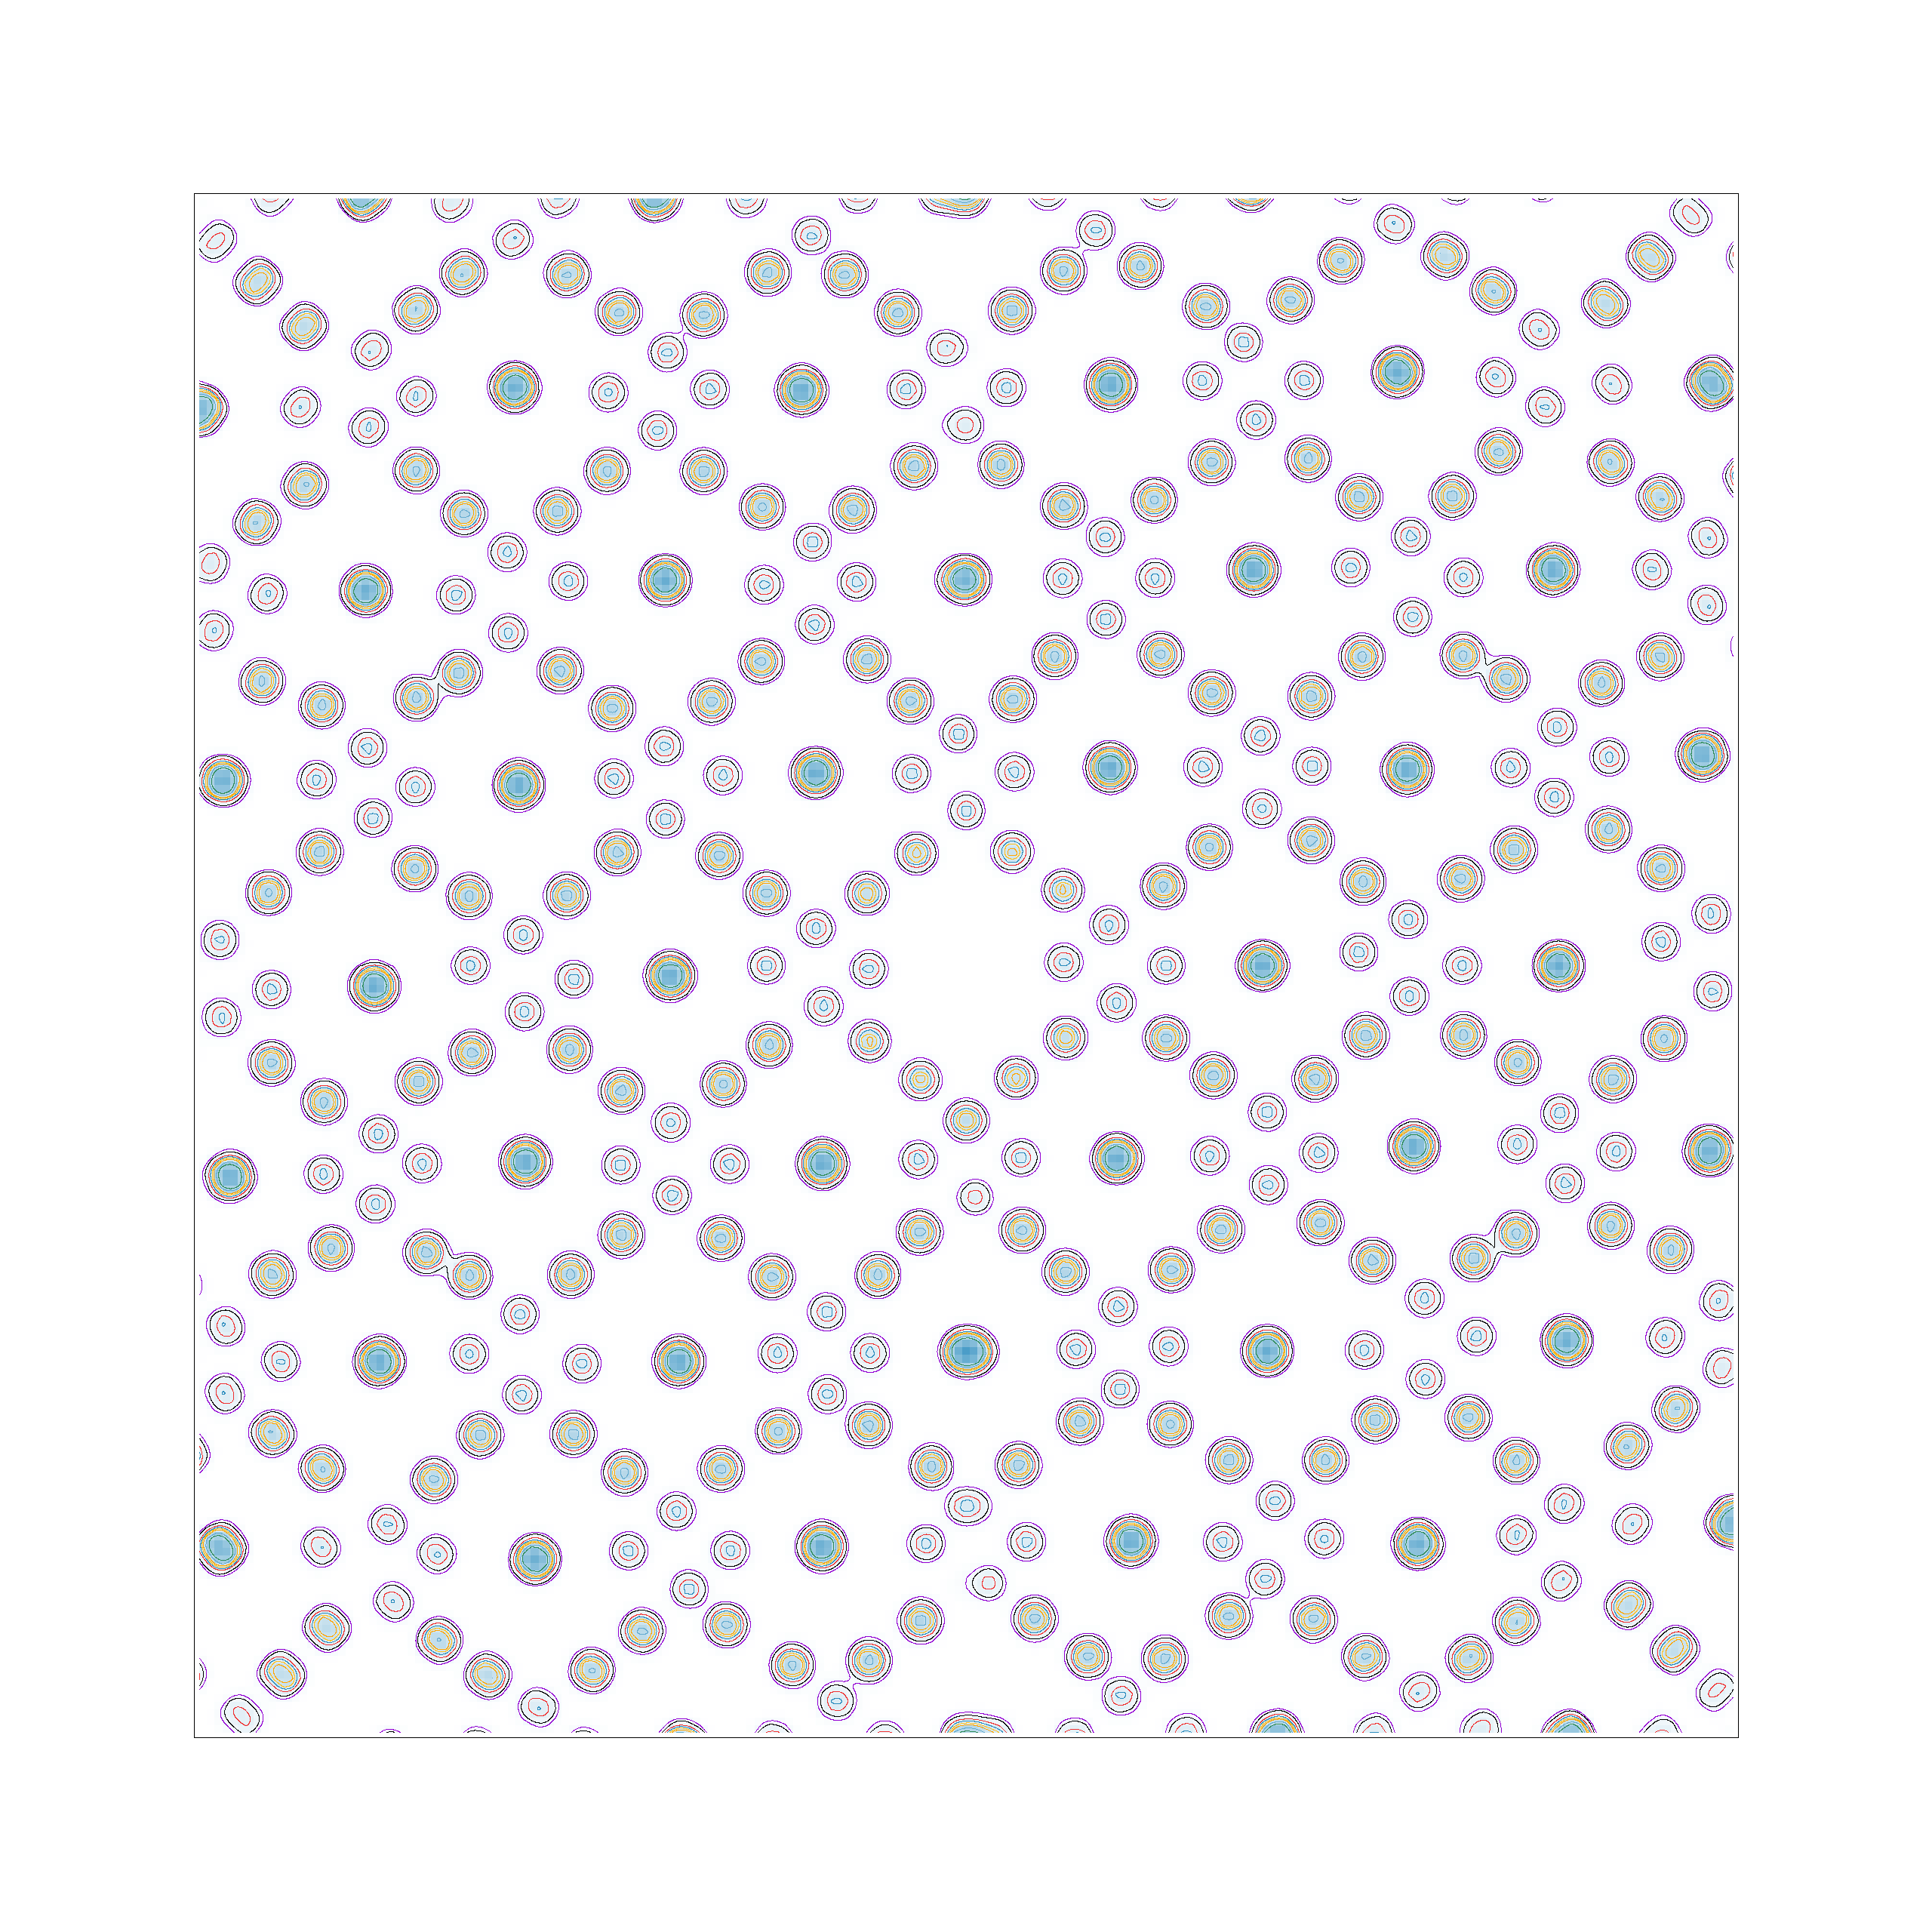
\includegraphics[width=\textwidth]{random-radial2d-part}
        \caption{Random radial2d}
        \label{fig:random radial2d}
    \end{subfigure}
    \caption{Comparison of crystalline and random assignment of bonds to a compact packing}
    \label{fig:compact bonds}
\end{figure}

\section{What Crystals would Form}

In the interests of developing more specialised tools for detecting crystalline order, we need to understand the crystal structures that are likely to form. This involves finding the structures that we believe to be the lowest in energy. To find these lowest energy structures we need tools other than molecular dynamics since the timescales for molecular dynamics are beyond the limits of our simulations. To find a good approximation of the lowest energy structures we look to packing hard shapes, by modelling our molecules as hard shapes we are able to use an isopointal algorithm to get a good approximation of the closest packed configurations. These closest packed configurations were then used as the starting configuration for a Lennard-Jones system. \texttabref{crystal energies} shows the energy of the Lennard Jones systems using the best packed isopointal structures for each wallpaper group as a starting configuration. The Lennard-Jones system does not retain the constraints of the wallpaper group symmetry, however the lower energy structures we are interested in do not deviate from these structures.

\begin{table}
    \sisetup{
        table-format = +3.4,
        table-omit-exponent,
        fixed-exponent =-4,
        parse-numbers=true,
        scientific-notation=true,
        round-mode=places,
        round-precision=3}
    \centering
    \begin{tabular}{ | l | S  S  S | }
        \hline
        {Crystal} & \multicolumn{3}{c|}{Energy per molecule (\num{e-4})} \\
            &\sone & \scon & \tri \\ \hline
        p1 & 0.00002598963975 & 0.0001551885511& -0.0003279078448\\
        p2 & 0.00001376280055& 0.0001527208398& -0.0003934685913\\
        p2mg & 0.000005732595806& 0.0004479052484& -0.0003354198174\\
        p2gg & 0.00002632511042& 0.0001699363766& -0.000401823091\\
        pg & 0.00002824743917& 0.0002860863393& -0.0004000561542\\
        p3 & 0.00003468842645& 0.0002424453316& -0.0003292839541\\
        \hline
    \end{tabular}
    \caption{Tabulated energies per particle}
    \label{tab:crystal energies}
\end{table}

From the energies in \texttabref{crystal energies} the most stable crystal structures are: \sone{} - p2mg, \scon{} - p2, and \tri{} - p2gg, with their repsectice configurations shown in \textfigref{crystals}. Interestingly these lowest energy structures are not necessarily the closest packed structures, it is possible the extra 

\begin{figure}
    \centering
    \begin{subfigure}[t]{0.47\textwidth}
        \includegraphics[width=\textwidth]{{{Snowman-0.4-0.637556-1.00-p2mg-frame}}}
        \caption{}
        \label{fig:crystal sone}
    \end{subfigure}
    \begin{subfigure}[t]{0.47\textwidth}%
        \includegraphics[width=\textwidth]{{{Snowman-0.4-0.637556-1.637556-p2-frame}}}
        \caption{}
        \label{fig:crystal sone}
    \end{subfigure}
    \begin{subfigure}{0.47\textwidth}
        \includegraphics[width=\textwidth]{{{Trimer-0.4-0.637556-1.00-120-p2gg-frame}}}
        \caption{}
        \label{fig:crystal sone}
    \end{subfigure}
    \caption{}
    \label{fig:crystals}
\end{figure}



\section{Order Parameters}


Rather than dealing with each molecule as at the start of this chapter we are now exploring order parameters of each individual particle, rather than each molecule.

One simple order parameter is to take the radial distribution function and apply it to each particle. Using each particle is going to be much closer to something seen in a x-ray defractometer as it is focused on center of density, rather than center of mass. These function still display the short range order...


We can also look at other properties of each particle, like the number of neighbours.

With the techniques that we possess we are unable to find any significant crystalline order in the system. There are small regions which show order, a result expected for a distribution of all possible arrangements, however these small regions are static, not displaying an important aspect of a crystal; growth.



